%!TEX root = ./Body.tex

\chapter{Ergebnise} % (fold)
\label{cha:Ergebnise}

\section{Online} % (fold)
\label{sec:Online}
Live-Test\\
.Unzureichende Performance. See figure ~\ref{fig:Ergebnis_Failed}.\\

\begin{figure}[htbp]
\begin{center}
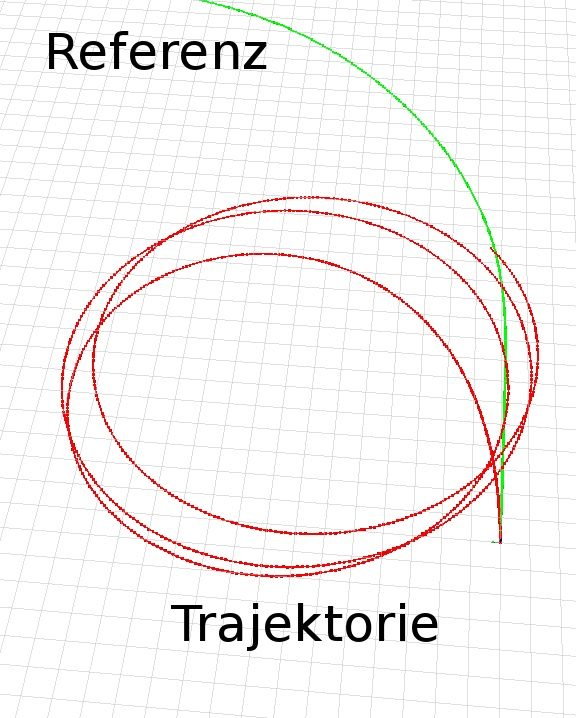
\includegraphics[width=0.5\textwidth]{Ergebnis_Failed}
\caption{Ergebnis Failedx}
\label{fig:Ergebnis_Failed}
\end{center}
\end{figure} 

Lenkung\\
.Feature-Raum\\
...Unzureichende Abdeckung mit Lerndaten\\
...Schlechte Generalisierung\\
See figure ~\ref{fig:Ergebnis_NN-winkel}.\\

\begin{figure}[htbp]
\begin{center}
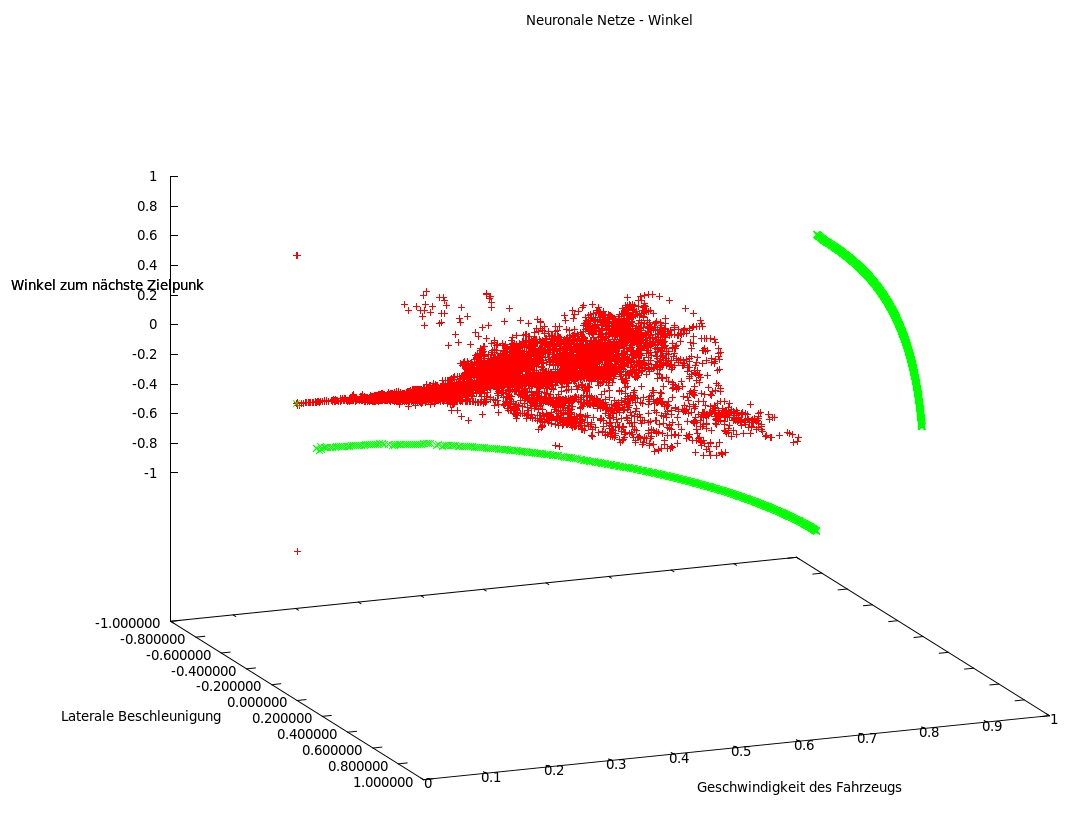
\includegraphics[width=0.5\textwidth]{Ergebnis_NN-winkel}
\caption{Ergebnis NN-winkel}
\label{fig:Ergebnis_NN-winkel}
\end{center}
\end{figure}

Gaspedal\\
.Feature-Raum\\
...Unzureichende Abdeckung mit Lerndaten\\
...Schlechte Generalisierung\\
See figure ~\ref{fig:Ergebnis_SVM-gas}.\\

\begin{figure}[htbp]
\begin{center}
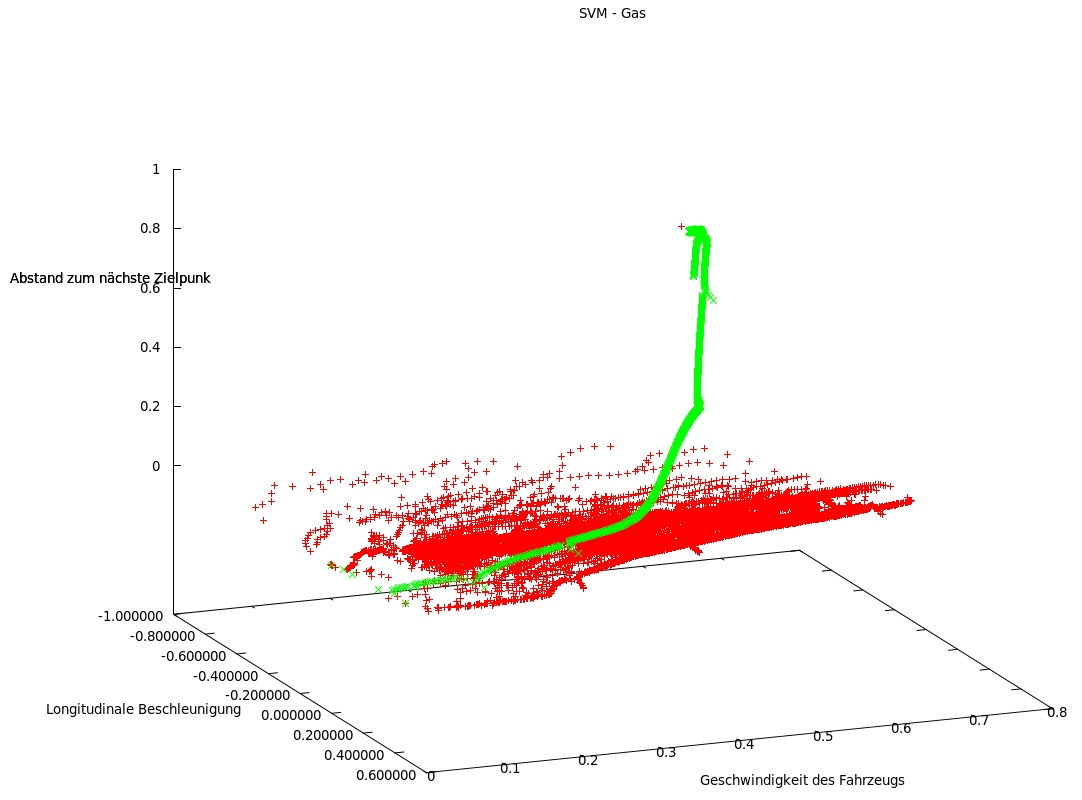
\includegraphics[width=0.5\textwidth]{Ergebnis_SVM-gas}
\caption{Ergebnis SVM-gas}
\label{fig:Ergebnis_SVM-gas}
\end{center}
\end{figure}
% section Online (end)


\section{Offline} % (fold)
\label{sec:Offline}
Evaluation\\
Abgleich der Ist- und Sollwerte\\
Sehr gute Performance\\
See figure ~\ref{fig:Ergebnis_x}.\\

\begin{figure}[htbp]
\begin{center}
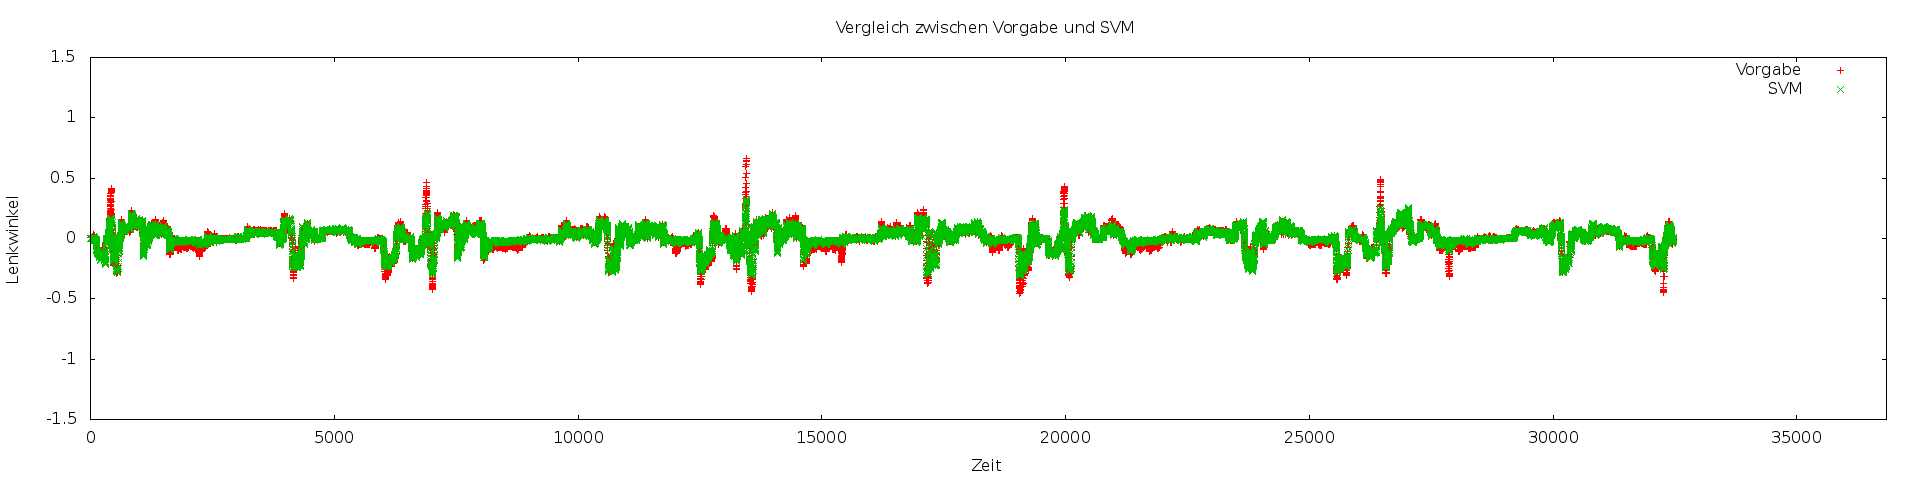
\includegraphics[width=0.5\textwidth]{Ergebnis_x}
\caption{Ergebnis x}
\label{fig:Ergebnis_x}
\end{center}
\end{figure}

Vergleich zwischen Soll- und Istwerten\\
Eingaben: Feature-Vektoren (Referenz)\\
Ausgaben: Stellgrößen (Lernverfahren)\\
Stellgröße (Referenz) zu Stellgröße (Lernverfahren)\\
See figure ~\ref{fig:Ergebnis_Evaluation}.\\

\begin{figure}[htbp]
\begin{center}
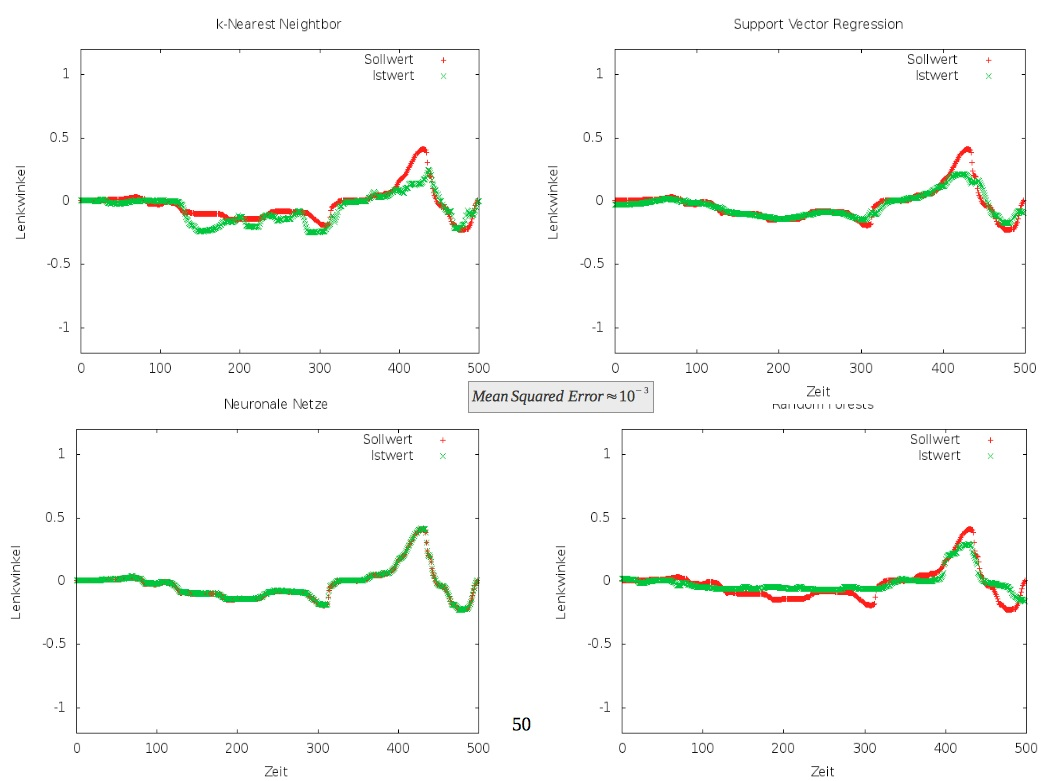
\includegraphics[width=0.5\textwidth]{Ergebnis_Evaluation}
\caption{Ergebnis Evaluation}
\label{fig:Ergebnis_Evaluation}
\end{center}
\end{figure}
% section Offline (end)


% chapter Ergebnise (end)
